\documentclass{projekt}
\usepackage[none]{hyphenat}
\usepackage{url}
\usepackage[utf8]{inputenc}
\usepackage[T1]{fontenc} 
\usepackage{ae}
\usepackage{fancyhdr}
\usepackage{graphicx}
\usepackage{pdfpages}
\usepackage[all]{xy}
\usepackage[czech]{babel}
\usepackage[activate={true,nocompatibility,all}, stretch=10, shrink=10, step=1, auto=true, draft=false]{microtype}
%\usepackage[total={17cm,28cm}, top=3cm, left=2cm, includefoot]{geometry}
\frenchspacing
\author{Filip Markvart}
\title{Datový model EEG/ERP portálu v prostředcích sémantického webu}
\titlet{} 
\titlett{}
\university{Západočeská univerzita v Plzni}
\faculty{Fakulta aplikovaných věd}
\department{Katedra informatiky a výpočetní techniky}
\subject{Diplomová práce}
\town{Plzeň}
\begin{document}
\pagestyle{fancy}
\renewcommand{\chaptermark}[1]{\markboth{\textit{#1}}{}}
\renewcommand{\sectionmark}[1]{\markright{\textit{#1}}{}}
\cfoot{\thepage}
\lhead{\leftmark}
\rhead{\rightmark}
\maketitle
\chapter*{Prohlášení}
\thispagestyle{empty}
Prohlašuji, že jsem diplomovou práci vypracoval samostatně a výhradně s~použitím citovaných pramenů.
\vskip 1.5em
V Plzni dne \today
\vskip 0.7em
\hskip 9cm Filip Markvart
\chapter*{Abstract}
\thispagestyle{empty}
\hspace{0.65cm}This thesis DODELAT
%describes a transformation of neuroinformatics metadata stored in the relational database to the semantic web standard. The main goal is to investigate existing tools and necessary %modifications that ensure automatic transformation for converting input data. The modified tool is able to process additional semantic information that cannot be stored in the relational %database.


%The last part describes design and implementation of an application that uses annotations to add semantic information to transformed data.

\tableofcontents
\pagestyle{fancy}
\renewcommand{\chaptermark}[1]{\markboth{\textit{#1}}{}}
\renewcommand{\sectionmark}[1]{\markright{\textit{#1}}{}}
\cfoot{\thepage}
\lhead{\leftmark}
\rhead{\rightmark}
\parskip 1em
\chapter{Úvod}
\hspace{0.65cm}EEG/ERP portál je webová aplikace sloužící výzkumným pracovníkům ke shromažďování a organizaci dat získaných při neuroinformatických experimen-\\tech v EEG laboratoři. Jejím cílem je ukládání naměřených dat v kontextu prováděného experimentu, který lze popsat rozsáhlou množinou různorodých údajů. Tato aplikace již prošla mnohaletým vývojem v jehož průběhu postupně docházelo ke změnám datového modelu kvůli přibývajícím požadavkům na uchovávaná data. Relační databáze jež slouží jako persistentní úložiště tak postupně byla rozšiřována o další tabulky, jejichž počet se k datu tvorby této práce pohybuje v řádu desítek. Většina realizací požadavků na ukládání dalších dat tak přímo znamená zásah nejen do databáze portálu ale také to do datové vrstvy, která ji využívá. V současné době tak databáze obsahuje velké množství tabulek uchovávající různá data, která jsou ale ve smyslu sémantiky často příbuzná a existuje mezi nimi vazba, která je prostřednictvím relačního datového modelu velmi obtížně popsatelná. Zároveň lze očekávat, že budou přibývat požadavky na uchování dalších dat, která navíc nemusejí mít jen homogenní strukturu (ve smyslu relační databáze), ale může se jednat i o množiny sémanticky příbuzných údajů – tzv. metadata, které budou vázány pouze k některým datům. Možnost ukládání strukturně heterogenních, ale sémantický příbuzných metadat je tak dalším otevřeným problémem.

Cílem této práce je prozkoumání struktury a nalezení sémantiky dat v současném datovém modelu relační databáze portálu a následná úprava tohoto modelu do podoby, která by dovolovala uchovat jak sémantiku dat, kterou není možné relačním modelem vyjádřit tak dodávat dynamicky datům přídavná metadata, aniž by muselo docházet k větším zásahům do datového modelu portálu. Pro realizaci úpravy datového modelu budou v této práci využity prostředky tzv. sémantického webu, který poskytuje množství standar-\\dů a technologií pro uchovávání organizaci a správu dat. Tyto technologie a nástroje zde budou popsány a na základě jejich analýzy budou vybrány prostředky, které se využijí pro implementaci úpravy zmiňovaného datového modelu. 
Poslední část práce se věnuje testování modifikovaného modelu a to především z výkonnostního hlediska. Díky této části by mělo být možné posoudit jak užitečnost samotné úpravy tak i použitelnost a efektivnost získaného modelu pro potřeby EEG/ERP portálu.


\chapter{Sémantický web}
\hspace{0.65cm}Dnešní podoba webu, tak jak je všeobecně známa, je tvořena značným množstvím informací, které mají řadu autorů, v podobě různých organizací či jednotlivců, jež se liší jak svým obsahem tak i podobou publikace. Tyto informace jsou poměrně snadno přístupné díky jejich jednoznačné identifikaci prostřednictvím URI identifikátoru (za předpokladu, že jej známe). K usnadně-\\ní získávání dalších (často příbuzných) informací napomáhají tzv. hypertexto-\\vé odkazy, jež usnadňují přístup k dalším zdrojům informací odstraněním požadavku na uživatelovu znalost identifikátoru cílového zdroje. Samotné hypertextové odkazy tak sice zajišťují provázání jednoho informačního zdroje s jiným díky znalosti jeho URI identifikátoru, ale nenesou už žádné další informace, které by například uživateli poskytly další údaje o cílovém zdroji. 
Takováto podoba umožňuje získávání informací jak koncovým uživatelům webu, tak v omezené podobě i vyhledávacím strojům, ale má své limity, neboť se v nepřeberném množství dat lze snadno ztratit, či se jen dostat k irelevantním informacím \cite{_1}.
Základním úkolem sémantického webu, jehož první myšlenky prezentoval v roce 2001 zakladatel konsorcia W3C Tim Berners-Lee, je umožnit aby informace dostupné prostřednictvím webu byly srozumitelné nejen uživatelům, ale také počítačům, jež tato data zpracovávají \cite{_2}. Hlavním cílem je tedy vývoj standardů a technologií, které by umožňovaly přesnější a podrobnější vyhledávání, integraci dat a také automatizaci častých úkonů. 
Sémantický web je založen na několika principech, které budou níže uvedeny.

\begin {itemize}

\item \textbf{Jednoznačná identifikace entit prostřednictvím URI}

\hspace{0.65cm}Veškerá data, reprezentující obvykle objekty reálného světa publikovaná prostřednictvím webu je možné jednoznačně odkazovat prostřednictvím identifikátoru URI. Díky této skutečnosti je tak možné realizovat i nepřímé odkazy na objekty, například osobu Petr Novák s emailem petr.novak@w3.org je možné identifikovat jako osobou, jejíž email má URI mailto:petr.novak@w3.org.


\item \textbf{Zdroje i odkazy mezi nimi je možné typovat}

\hspace{0.65cm}Současná podoba webu je tvořena zdroji a odkazy jež je vzájemně propojují. Zdroje, které jsou reprezentovány webovými dokumenty jsou publikovány za účelem poskytnutí informací lidskému uživateli, který dokáže ze samotného obsahu dokumentu získat i některá jeho metadata (pokud jsou v určité formě součástí obsahu) a do jisté míry také vztah k ostatním dokumentům, na něž vedou případné odkazy. Stroje v podobě různých vyhledávačů či automatů pro shromažďování dat ale tuto schopnost nemají nebo je pro ně příliš náročná. Řešením sémantického webu je typování jak samotných zdrojů, tak i odkazů, které je provazují. Díky této skutečnosti je pak možné webovým dokumentům dodávat metadata jako např. autora, verzi či závislost na jiném dokumentu. Z hlediska typování odkazů je například možné jeden webový zdroj označit pouze jako odlišnou verzi jiného zdroje.


\item \textbf{Tolerance neúplných informací}

\hspace{0.65cm}U současně podoby webu může nastat situace, kdy některý zdroj není dostupný. V takovém případě uživatel ztrácí přistup k danému dokumentu, ale díky koncepci webu není nikterak ohrožena dostupnost ostatních zdrojů. V případě sémantického webu se situace nemění, nedostupnost některého zdroje není žádnou překážkou, neboť nástroje sémantického webu zpracovávají pouze ty informace, které jsou dostupné a těch vytvářejí závěry. V důsledku je tak možné dojít při zpracovávání dat ke stejným výsledkům, jako v případě, když jsou zpracovávány jen některé vybrané informace, jejichž rozsah je explicitně definován.

\item \textbf{Zpracování neověřených dat}

\hspace{0.65cm}Při zpracování informací pocházejících z neověřených zdrojů je možné dohledávat prostřednictvím typovaných odkazů důvěryhodná data, jejichž obsah a odkazy poslouží jako ověřovací prostředek. Tento princip je možné uvést na jednoduchém příkladu. Aplikace zpracovávající data sémantického webu vyhledá informace, přičemž je kladen požadavek na vysokou pravděpodobnost správnosti výsledku. Pokud část nalezených informací pochází z neověřeného zdroje, je možné vyhledávat například jejich autora v odkazech zdrojů, které jsou důvěryhodné. V případě úspěchu nalezení takového odkazu u více různých zdrojů je pak možné považovat zkoumaný zdroj s vysokou pravděpodobností rovněž za důvěry-\\hodný a tím zajistit plnění požadavků na výsledek.

\item \textbf{paralelního vývoje dat}

\hspace{0.65cm}V průběhu času nezřídka nastávají situace, kdy autoři, či skupiny autorů publikují obdobná data na různých místech nebo v odlišném čase. Obsah těchto dokumentů se může navíc lišit svým jazykem či použitou terminologií, ač význam bude shodný. S využitím prostředků sémantického webu je ale možné prostřednictvím typovaných odkazů zajistit provázanost významově obdobných či na sebe navazujících dat i přes překážku rozdílnosti jejich podoby zápisu. Navíc je také možné dodávat nové informace bez nutnosti úpravy původních dat, která tím pádem nezmění svoji strukturu \cite{_1}.

\end{itemize}


\section{Architektura sémantického webu}
\hspace{0.65cm}Architektura sémantického webu sestává z více oddělených vrstev, mezi nimiž je zajištěna zpětná i dopředná kompatibilita \cite{_3}. Nejnižší vrstva je tvořena dvěma technologickými standardy – URI identifikátory sloužící pro jednoznačné pojmenování zdrojů dat a Unicode kódování mezinárodní znako-\\vou sadou. Druhou vrstvu architektury, jež je patrná z obrázku 2.1, reprezentu-\\je značkovací jazyk XML (Extensible Markup Language), který umožňuje tvorbu strukturovaného dokumentu za užití vlastních značek. Tato vrstva zároveň zajišťuje definici XML schématu včetně jmenných prostorů. RDF + rdfschema jež následuje je klíčovou vrstvou sémantického webu neboť dovoluje tvorbu vazeb a vztahů mezi jednotlivými zdroji, které jsou typované spolu s odkazy. Je tak možné definovat libovolné vztahy mezi objekty či jejich kategoriemi bez nutnosti specifikace významu samotných vazeb či objektů. Díky RDF schématu je vytvářena základní sémantika datového modelu, která už definuje význam některých elementů jako třídy či podtřídy. 
Vrstva ontologického slovníku, zastoupená jazykem OWL, nabízí pokročilou reprezentaci znalostí na úrovni deskripční logiky a umožňuje tak vytvářet složitější struktury sloužící k popisu různých vlastností objektů \cite{_2}. Poslední vrstvou, která je jako všechny předchozí zmíněné konsorciem W3C standardizo-\\vaná jsou digitální podpisy. Ty poskytují možnosti například pro detekci různých verzí dokumentů. Zbylé výše znázorněné vrstvy slouží pro definice a vyhodnocování odvozovacích pravidel a v současnosti jsou ve fázi vývoje \cite{_1}.

\begin{figure}[htb]
\begin{center}
\includegraphics[scale=0.62]{architektura.pdf}
\caption{Architektura sémantickém webu \cite{_1}}
\end{center}
\end{figure}

Vrstvení jazyků sémantického webu je podstatné pro úroveň expresivity znalostního modelu, neboť s rostoucí vyjadřovací možností jazyka také roste složitost dotazovacích operací nad modelem. Je tedy nutné před započetím tvorby modelu nejprve zjistit jeho požadovanou expresivitu a podle té zvolit pro zápis dat jazyk, který ji dovoluje obsáhnout. Využívá se tedy skutečnosti, že jazyk vyšší vrstvy zahrnuje vyjadřovací schopnosti vrstev nižších\cite{_2}. 
Další podkapitoly se budou zabývat podrobněji jednotlivý zmíněnými technologiemi.

\section{XML}
\hspace{0.65cm}XML (eXtensible Markup Language) je značkovací jazyk sloužící pro popis hierarchických struktur textových dokumentů prostřednictvím tzv. tagů. Tag je konstrukce, která slouží k počátečnímu a koncovému ohraničení společně definovaného elementu. Tag lze chápat jako prostředek pro dodání metadat ke textové struktuře, jež ohraničuje. Příkladem může být následující zápis {\it <prijmeni>Novák</prijmeni>}, kde elementu {\it Novák} je dodána meta informace, že se jedná o příjmení. Samotné XML ale nedefinuje žádný sémantický význam tagů, slouží pouze pro specifikaci syntaxe na úrovní XML dokumentu. Pro definici (zejména hierarchické) struktury XML dokumentu slouží XML Schema, které umožňuje zápis pravidel, jež musí cílový dokument dodržovat pro zachování své validity. Ze strany sémantického webu ale nemají pravidla XML Schema žádný sémantický význam a slouží tak pouze pro definici struktury a syntaxe. Zmíněné schéma také definuje základní datové typy (čísla, řetězce, čas a pod.), které nabývají významu v sémantických jazycích jako je RDF \cite{_3}.


\section{RDF}
\hspace{0.65cm}Technologický základ sémantického webu tvoří jazyk RDF (Resource Description Framework), jež slouží jako obecný rámec pro popis, výměnu a opětovné použití metadat \cite{_3}. Tento rámec poskytuje jednoduchý model sloužící pro popis zdrojů jež je nezávislý na jeho konkrétní implementaci \cite{_4}. Samotné informace o objektu jsou realizovány prostřednictvím tvrzení, jež se označují jako trojice (anglicky triple). Každou trojici tvoří spolu subjekt, predikát a objekt. Subjekt je libovolný objekt identifikovatelný pomocí URI, který se snažíme prostřednictvím trojice popisovat, zaznamenat nějakou jeho vlastnost. Tato vlastnost se popisuje prostřednictvím predikátu, který vede ve směru od subjektu ke objektu, přiřazuje tedy subjektu nějaký objekt prostřednictvím této vlastnosti. Cílový objekt pak představuje hodnotu, které předchozí objekt nabývá pro daný predikát. 
Tento princip je možné znázornit na jednoduchém tvrzení, zapsaném větou „Martin staví dům.“ Subjektem trojice potom bude Martin, predikátem staví a objektem dům, tak jak je znázorněno na obrázku 2.2. 
\\
\vspace{0.1cm}

\begin{figure}[htb]
\begin{center}
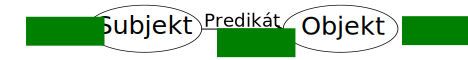
\includegraphics[scale=0.9]{trojice.pdf}
\caption{Příklad RDF trojice}
\end{center}
\end{figure}

Dle definovaného standardu \cite{_5} je možné, aby objektem byl jiný subjekt. Díky této skutečnosti je možné jednotlivé trojice spojovat do většího celku, který ve výsledku tvoří strukturu orientovaného grafu, kterou lze označit jako model \cite{_3}. Jednoduchým model tvořený dvěma trojicemi lze vytvořit využitím dalšího tvrzení „Dům stojí v Plzni.“ V předchozí trojici pak bude dům subjektem namísto objektu a dojde tak ke spojení dvou trojic (za předpokladu že v obou tvrzeních je myšlen stejný fyzický dům), tak jak je znázorněno na obrázku 2.3. 

\begin{figure}[htb]
\begin{center}
\includegraphics[scale=0.9]{miniStrom.pdf}
\caption{Příklad jednoduchého RDF modelu}
\end{center}
\end{figure}


Z hlediska implementace mohou být uzly orientovaného grafu datového modelu tvořeny URI identifikátorem, anonymním listem nebo literálem \cite{_6}. URI identifikátor obsahuje pouze adresu zdroje v textové podobě ve znakové sadě Unicode a zastupuje tak konkrétní jedinečný objekt. Anonymní list (anglicky blank node) je prvek nahrazující URI identifikátor při absenci unikátní adresy zdroje. Tato entita přestavuje zdroj, který je sice v rámci grafu popisován prostřednictvím trojic, ale není potřeba (často z hlediska významu), aby byl dostupný i vně grafu. S URI má společné to, že musí nést adresu zdroje (její syntaxe není implicitně definována), ale liší se skutečností, že tato adresa musí být unikátní pouze v rámci obalujícího modelu, nikoliv vně grafu. Může tak nastat situace, že dva odlišné modely budou obsahovat (ze syntaktického hlediska) dva stejné anonymní uzly, což v případě URI možné není (při respektování specifikace). Tento list tak může představovat anonymní objekt sloužící ke vytvoření vazby mezi jinými objekty, které jsou z hlediska sémantiky významné \cite{_5}. Jako příklad je možno uvést následující tvrzení. „Martinův přítel zná předpověď počasí. Počasí bude deštivé.„ Zjednodušeným převodem předchozích vět na trojice v podobě subjekt – predikát – objekt získáme: Martin – má – přítel, přítel – zná – počasí, počasí – bude – deštivé. 
Subjekt resp. objekt přítel zde může být reprezentován anonymním listem, v případě že jedinou signifikantní informací (z vnějšího pohledu na datový model) je Martinova získaná znalost počasí, nikoliv už jeho přítel, jež mu ji zprostředkoval. 
Poslední možnou reprezentací entity trojice je literál, jež nese Unicode textový řetězec, který slouží pro zápis koncové informace (užitečné pro lidského čtenáře). Literál může také navíc obsahovat položku, pro označení jazyka, ve kterém je textová informace zapsána \cite{_6}. 
\\
\\
Pro komponenty každé trojice grafu platí následující pravidla \cite{_6}.

\begin {itemize}

\item \textbf{subjekt} - může být tvořen URI identifikátorem nebo anonymním listem
\item \textbf{predikát} - může být tvořen pouze URI identifikátorem
\item \textbf{objekt} - může být tvořen URI, anonymním listem nebo literálem

\end{itemize}


Pro zápis trojic RDF grafu je sice možné využít grafické podoby, ale pro vyjádření sémantiky webových zdrojů je nejvhodnější využít syntaxe jazyka XML. Níže uvedená ukázka kódu reprezentuje XML zápis trojice z obrázku 2.2.

\begin{verbatim}
<rdf:RDF xmlns:rdf="http://www.w3.org/1999/02/22-rdf-syntax-ns#"
         xmlns:dc="http://purl.org/dc/elements/1.1/">
  <rdf:Description rdf:about="http://www.w3.org/Person/Martin">
    <dc:stavi>dům</dc:stavi>
  </rdf:Description>
</rdf:RDF>

\end{verbatim}

Samotné RDF nedefinuje trojicím ani jejím částem sémantiku, ale dovoluje vyjádřit základní vztahy náležitosti prvků do kategorie prostřednictvím kontej-\\nerů a kolekcí (např. rdf:Bag, rdf:List) \cite{_2}. Pro dodání základní sémantiky slouží schéma popsané v následující podkapitole.

\section{RDFS}
\hspace{0.65cm}RDF Schema (Resource Description Framework Schema) funguje jako základní jazyk pro tvorbu ontologií s velmi jednoduchou sémantikou. Toto schéma rozšiřuje jazyk RDF o možnosti vyjádření vlastností objektů, konstruk-\\ce tříd objektů a popis jejich hierarchie \cite{_2}. 
Prostředky jazyka RDFS umožňují především vyjádření vztahů mezi zdroji a lze je rozdělit na dvě skupiny – třídy a vlastnosti.

\subsection{Třídy}
Skupiny zdrojů je možné rozčleňovat do skupin označovaných jako třídy (classes), jejichž členové se nazývají instance třídy. Na úrovni RDFS se rozlišují třídy od svých instancí a každá třída jich může mít neomezený počet. Dvě třídy mohou mít navíc shodnou množinu instancí tříd a zároveň tyto třídy mohou být navzájem různé. Bude-li se tedy například definovat třída {\it A} jako osoby pracující v kanceláři {\it 1} a třída {\it B} jako osoby žijící ve městě {\it X}. Potom je možné aby různé třídy {\it A} a {\it B} měly stejné množiny instancí, za předpokladu, že každá osoba pracující v kanceláři {\it 1} bydlí ve městě {\it X}. Pro třídy platí také dědičnost – bude li třída {\it B} podtřídou {\it A}, pak všechny instance {\it B} jsou zároveň instancí třídy {\it A}. Koncept tříd RDFS definuje následující konstrukce \cite{_7}:

\begin {itemize}

\item \textbf{rdfs:Resource} představuje RDF zdroj, který je obalující třídou všech prvků – je tedy nejvýše postavenou rodičovskou třídou, {\it rdfs:Resource} je zároveň instancí {\it rdfs:Class}
\item \textbf{rdfs:Class} reprezentuje rodičovskou třídu všech RDF tříd zdrojů, čímž je {\it rdfs:Class} instancí {\it rdfs:Class} (sebe sama)
\item \textbf{rdfs:Literal} třída je instancí {\it rdfs:Class}, která slouží pro reprezentaci RDF literálů a je podtřídou {\it rdfs:Resource}
\item \textbf{rdfs:Datatype} je obalující třídou pro datové typy, které jsou její instancí, {\it rdfs:Datatype} je zároveň podtřídou i instancí {\it rdfs:Class} a každá její instance je podtřídou {\it rdfs:Literal}
\item \textbf{rdf:XMLLiteral} je třída XML literálů, která je podtřídou {\it rdfs:Literal} a instancí {\it rdfs:Datatype}
\item \textbf{rdf:Property} představuje rodičovskou třídu všech definovaných vlastností a je instancí {\it rdfs:Class}


\end{itemize}


\subsection{Vlastnosti}
\hspace{0.65cm}Vlastnosti (properties) slouží k vyjádření vztahu mezi dvěma zdroji – na úrovni trojice mezi subjektem a objektem. Koncept RDFS definuje následující vlastnosti:

\begin {itemize}


\item \textbf{rdfs:range} je instancí {\it rdf:Property}, která slouží ke vyjádření, že objekt jehož predikát má definovaný {\it  rdfs:Range X} bude zároveň instancí {\it X}, například z následujících trojic {\it A – rdfs:Range B a X – A – C} bude vyplývat, že {\it C} je instancí {\it B}, 
zároveň platí, že objekt s definovaným predikátem může být instancí více tříd (pokud má predikát definováno více {\it  rdfs:Range}).

\item \textbf{rdfs:domain} představuje instanci {\it rdf:Property}, která vyjadřuje, že zdroj (subjekt) jehož predikát má definovaný {\it rdfs:Domain X} bude také instancí {\it X}, tento zdroj může být jako v předchozím případě instancí více tříd při definování více {\it rdfs:Domain}
\item \textbf{rdf:type} slouží k definování, že zdroj (subjekt) je instancí třídy definované objektem, pokud tedy platí {\it A rdf:type B}, pak {\it A} je instancí {\it B}
\item \textbf{rdfs:subClassOf} je vlastnost sloužící k vyjádření náležitosti instancí jedné třídy jako instancí jiné třídy, pokud platí {\it A rdfs:subClassOf B}, pak {\it A} je podtřídou {\it B} a všechny instance třídy {\it A} jsou zároveň instancí třídy {\it B}, tato vlastnost je navíc tranzitivní, takže popsanou dědičnost je možné řetězit do libovolné délky
\item \textbf{rdfs:subPropertyOf} slouží k vyjádření dědičnosti vlastností, pokud platí {\it P1 subproperty P2}, pak pro trojici {\it A P1 B} platí, že subjekt {\it A} má pro vlastnost {\it P1} i {\it P2} pro objekt {\it B}
\item \textbf{rdfs:label} umožňuje zdroji (subjektu) přidat textovou informaci jako lidsky čitelnou náhradu pro označení zdroje
\item \textbf{rdfs:comment} dovoluje přidat zdroji popisek, který usnadňuje lidskému uživateli pochopit význam zdroje \cite{_7}

\end{itemize}

Vyjádření vztahů mezi jednotlivými vlastnostmi a třídami je patrné z obrázku 2.4. Rámec RDFS dále ještě definuje vlastnosti a třídy pro kontejnery a kolekce, které je možné naleznout ve \cite{_7}.

\begin{figure}[htb]
\begin{center}
\includegraphics[scale=1.4]{rdfs.pdf}
\caption{Vztahy mezi vlastnosmi a třídami RDFS}
\end{center}
\end{figure}

\section{Ontologie}
\hspace{0.65cm}Znalostní modely, jež jsou popisované vyššími jazyky sémantického webu se označují jako ontologie. Ontologie ovšem není pouze abstraktním znalostním modelem, ale slouží i jako prostředek pro k získání interoperability, tedy schopnosti vzájemné spolupráce oddělených systémů na úrovni sdílení dat a poskytování služeb \cite{_2}. Definicí ontologie v informatice jež uvádí Thomas Gruber, zakladatel ontologického inženýrství, je „formální specifikace sdílené konceptualizace“\cite{_8}. V této definici je formálností myšleno vyjádření znalostí prostřednictvím jazyka s formálním a logickým základem. Pojem konceptualizace znamená definování konceptů na dané úrovni abstrakce, jež odpovídá požadavkům pro model domény. Tuto doménu pak vytvářejí osoby, pro které je daná ontologie závazně (vzájemnou dohodou) definovaná jako prostředek pro popis dat, jež musejí všichni členové dodržovat \cite{_2}. V důsledku se tak jedná o tvorbu abstraktního modelu v určené oblasti, kde se definují pojmy společně se vzájemný vztahy vyjádřené logickým jazykem. Cílem explicitní specifikace pojmů a vztahů je snaha o porozumění znalostně orientovaných systémů \cite{_9}.
Ontologie lze z hlediska vývoje rozčlenit do tří kategorií:

\begin {itemize}

\item \textbf{Terminologické (lexikální)} Slouží především ke zachycení taxonomie definovaných pojmů a popis jejich vzájemných vztahů, jejich realizace se často podobá slovníkům synonym.
\item \textbf{Informační} Zastávají roli služby stojící nad databází, která zajišťuje vyšší míru abstraktnosti při databázovém dotazování.
\item \textbf{Znalostní} Dovolují reprezentaci znalostí především v oblasti umělé inteligence, kde jsou chápány jako logické teorie, jejichž elementární prvky se definují prostřednictvím formálního jazyka. Využívají se zejména ve znalostně orientovaných systémech \cite{_10}.

\end{itemize}

Dle míry formalizace a cílového předmětu konceptualizace se rozlišují 4 kategorie ontologie.

\begin {itemize}

\item \textbf{Doménové} Zabývají se specifikací určité oblasti – domény.
\item \textbf{Generické} Blíží se svou podobou doménovým, ale pokrývají širší množinu dat a zachycují tak obecnější koncepty, nejdou ovšem do příliš velké hloubky. Popisují například realitu prostřednictvím vzájemných časoprostorových pozic objektů. Často se snaží zachytit všeobecné znalosti, které odpovídají běžně používaným lidským vědomostem.
\item \textbf{Úlohové} Tyto ontologie jsou zaměřené zejména na odvozovací procesy namísto záznamu znalostí a slouží především jako modely pro řešení určitých problémů – např. pro diagnostiku či plánování.
\item \textbf{Aplikační} Jsou většinou vázány na specifické aplikace, kde spojují doménovou a úlohovou ontologií \cite{_10}.
\end{itemize}

Pro realizaci popsaných ontologií je zapotřebí jazyka, který by dovoloval formální zápis. Výše uvedené schéma RDFS je z hlediska sémantického webu základní podobou ontologie, kterou je dále možné rozšiřovat například s využitím jazyků jako je OWL.


\section{OWL}
\hspace{0.65cm}OWL (Web Ontology Language) je jazyk sémantického webu navržený pro získávání a zpracování informací prostřednictvím strojů (aplikací), namísto současného stavu, kdy jsou informace určeny pouze pro lidské uživatele. Tento jazyk využívá technologií XML, RDF a RDFS jakožto primárních prostředků pro tvorbu ontologických slovníků se základní sémantikou, kterou sám dále rozšiřuje o možnosti vyjádření složitějších výrazů a jejich vzájemných vztahů \cite{_11}. Mezi tato rozšíření patří například kardinalita, univerzální a existenční kvantifikace, matematické charakteristiky vlastností jako např. tranzitivnost, disjunktnost či inverze a anonymní třídy (sloužící  často k jednorázovému využití) \cite{_12}.
Vzhledem k tomu, OWL nabízí poměrně pokročilou úroveň expresivity jazyka, je nutné brát v potaz výpočetní složitost algoritmů odvozo-\\vacích a usuzovacích nástrojů pracujících s vytvořenou ontologií. Z tohoto důvodu jsou specifikovány 3 varianty jazyka OWL, které se vzájemně liší mírou expresivity \cite{_2}.


\begin {itemize}

\item \textbf{OWL Lite} Umožňuje definovat hierarchický systém tříd s jednoduchými omezeními vazeb \cite{_11}. Dále poskytuje prostředky pro zaznamenání syme-\\trické, transitivní a inverzní vlastnosti a také jednoduchá omezení na velikosti množin vybraných objektů modelu – kardinalitu, která je ale v této verzi omezena pouze na přípustné hodnoty 0 a 1 \cite{_2}.
\item \textbf{OWL-DL} Tato varianta poskytuje maximální možnou expresivitu jazyka, u které je stále splněna podmínka rozhodovací úplnosti (jakékoliv rozhodovací pravidlo je možné použít na kteroukoliv část ontologie) a výpočetní splnitelnosti (veškeré výsledky odvozovacích operací budou získány v konečném čase) \cite{_2}. OWL-DL nabízí veškeré konstrukce jazyka OWL, které ale podléhají určitým omezením při jejich použití, např. není možné využít omezení kardinality pro vlastnosti definované jako tranzitivní. Z hlediska množiny dostupných jazykových konstrukcí dovo-\\luje tato varianta oproti OWL Lite definovat navíc sjednocení, disjunkce a doplňky tříd nebo libovolné omezení kardinality \cite{_11}.
\item \textbf{OWL-Full} Je variantou, která poskytuje maximální možnou expresivitu, ke které využívá stejně jako předchozí verze všech konstruktů jazyka OWL. Tato varianta neklade žádná omezení pro vyhodnocovací pravidla, díky čemuž ale není možné zaručit výpočetní splnitelnost. OWL-Full dovoluje ještě navíc uživatelskou změnu sémantického významu nativně definovaných konstrukcí jazyků RDF a OWL. Tato verze ovšem není prakticky příliš využitelná, neboť v současnosti nejsou známé žádné efektivní algoritmy, které by dovolovaly nad modelem dat provádět usuzovací operace využívající všech vlastností OWL-Full \cite{_2}.

\end {itemize}

Každá verze OWL je rozšířením svého předchůdce díky čemuž je ontologie vyjádřená v jednodušší variantě platná i pro verzi vyšší, např. tedy každá ontologie zapsaná ve OWL Lite bude plně validní ve OWL-DL (což ale obráceně neplatí) \cite{_11}.
Mezi typické odvozovací úlohy v kontextu OWL patří například odvozování taxonomické struktury, ověřování příslušnosti instance ke třídě, klasifikace individuí vzhledem k definované ontologii či testování splnitelnost logické teorie \cite{_12}.


\section{SPARQL}
\hspace{0.65cm}Základním prostředkem pro dotazování nad daty sémantického webu je jazyk SPARQL (SPARQL Protocol and RDF Query Language). Tento jazyk standardizovaný konsorciem W3C umožňuje vytvářet dotazy nad RDF grafy prostřednictvím vzorů RDF trojic spolu s logickými operacemi konjunkce a disjunkce \cite{_2}. Konstrukce těchto dotazů je sice složitější než v případě SQL dotazů nad relačními databázemi, ale umožňuje ze zdrojové ontologie získávat komplexnější informace \cite{_3}. SPARQL dotaz se skládá ze 3 základních částí. První část – označovaná jako prolog slouží k definování jmenných prostorů a prefixů, které budou v dalších částech dotazu použity. Druhou částí je hlavička dotazu, kde se určuje jaký typ dotazu se bude v další části provádět. Třetí a hlavní část SPARQL slouží k definování cílové ontologie (RDF grafu) pro dotazování (v případě, že cílový graf je implicitně definován, je tato část vynechána) a proměnných včetně samotných vyhledávacích podmínek v podobě grafových vzorů (graph pattern)\cite{_2}.
Tento jazyk částečně vychází ze SQL, což je patrné i na jeho syntaxi. Např. klauzule FROM slouží pro výběr cílového grafu pro dotazování, či klíčové slovo WHERE slouží pro uvození zápisu souboru RDF trojic – tzv. grafového vzorce, jež je jádrem dotazu. Vyhodnocování dotazu poté probíhá takovým způsobem, že dochází k porovnávání grafového vzorce se s RDF daty \cite{_13}. 
Pro názornost je níže uveden zápis jednoduchého SPARQL dotazu, který slouží k vyhledání jmen a příjmení všech osob v implicitně zadaném grafu.

\begin{verbatim}
PREFIX zcu: <http://www.zcu.cz/ns/students>
SELECT ?name ?surname
WHERE  {
     ?person x zcu:Person.
     ?person zcu:Name ?name.
     ?person zcu:Surname ?surname
}
\end{verbatim}


SPARQL podporuje 4 druhy dotazů, které se vzájemně liší v typu vráceného výsledku \cite{_13}.

\begin {itemize}

\item \textbf{SELECT} Tento typ dotazu nejvíce odpovídá běžnému SQL dotazování, neboť zadaným proměnným nastaví příslušné hodnoty a vrací je v podobě tabulky \cite{_14}.
\item \textbf{ASK} Dotaz typu ASK vrací pouze boolean odpověď a slouží ke otesto-\\vání, zda zadaný grafový vzorec má pro daný graf řešení. ASK tak slouží ke testování vytvořených logických hypotéz, ale neumožňuje už vrácení konkrétních řešení \cite{_13}.
\item \textbf{DESCRIBE} Dotazy typu DESCRIBE navrací podgraf dotazovaného grafu, který obsahuje všechny dostupné informace o zdroji, jež vyhověl zadanému grafovému vzoru \cite{_13}. Při vyhodnocování dotazů dochází k porovnávání zdrojů získaných ze vstupního grafového vzoru se zdroji celého grafu. Pro nalezené odpovídající zdroje jsou pak získány všechny vázané relevantní informace, ze kterých je ve výsledku složen navracený graf \cite{_14}.
\item \textbf{CONSTRUCT} Tento speciální druh dotazu navrací jako výsledek nový RDF graf dle definované grafové šablony. Výsledný RDF graf je konstruován podle částečných řešení dotazovací sekvence, jež vyplňují proměnné ze zadané grafové šablony na základě které jsou tvořené výsledné trojice pro cílový navracený graf \cite{_13}. Tato dotazovací operace se do jisté míry podobá XSLT transformaci XML dokumentu.

\end {itemize}

\chapter{EEG/ERP portál}


\bibliography{diplomka}
\bibliographystyle{plain}


\end{document}
